\begin{frame}{Standard e tecnologie: Sommario}
	\begin{itemize}
		\item Tecnologie di comunicazione
		\begin{itemize}
			\item IEEE 802
			\begin{itemize}
				\item Ethernet
				\item Wireless
				\item Bluetooth
				\item ZigBee \& 6LoWPAN
				\item WiMAX
			\end{itemize}
			\item Power Line Communication
		\end{itemize}
		\item Standard per lo scambio di informazioni
		\begin{itemize}
			\item Modbus
			\item ISO/IEC 61850
		\end{itemize}
		\item Standard per la sicurezza
		\begin{itemize}
			\item ISO/IEC 62351
		\end{itemize}
	\end{itemize}
\end{frame}

\plain{Tecnologie di comunicazione}
\begin{frame}{IEEE 802}
	\begin{itemize}
		\item Famiglia di standard sviluppati per il supporto alle reti locali
		\item L'architettura è incentrata sui due livelli inferiori del modello ISO/OSI
	\end{itemize}
	\begin{figure}[h] 
		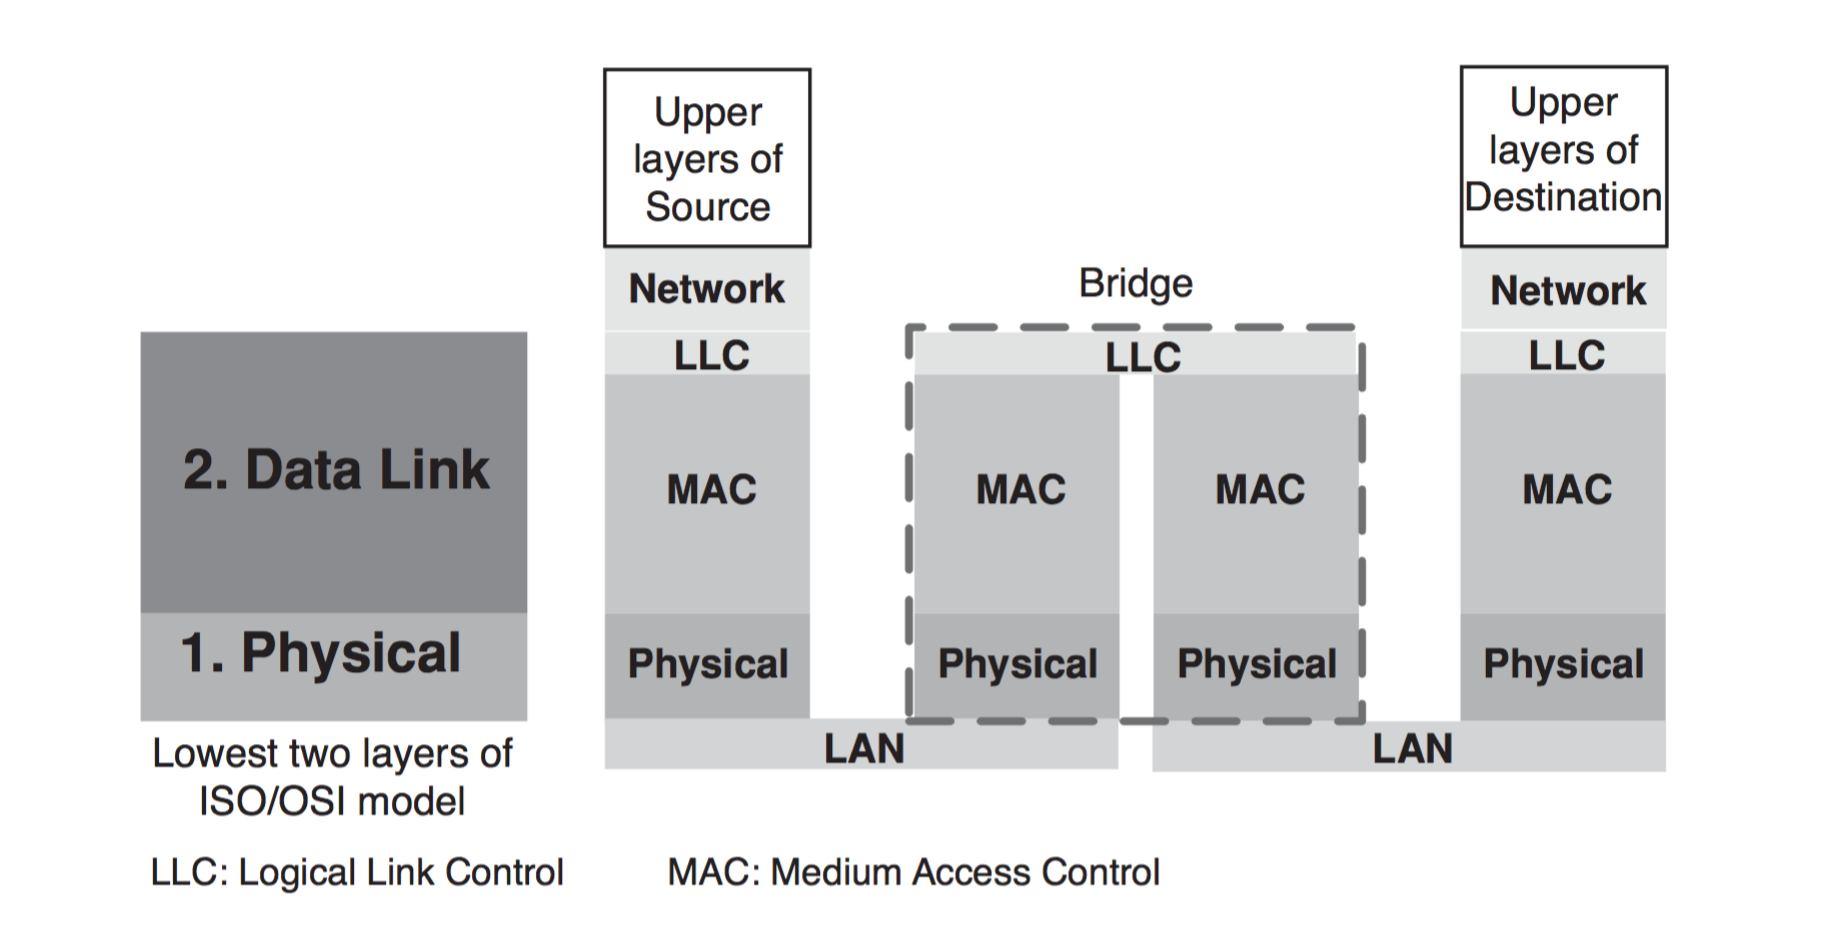
\includegraphics[scale=0.3,cfbox=blue_slides 1pt 0pt]{imgs/arch_ieee802.png}
	\end{figure}
\end{frame}

%Un set di host connessi ad una rete in modo tale che la trasmissione simultanea da due host nel set porta a collisioni, crea un dominio di collisione. Inoltre, le LAN Ethernet trasportano anche frame di broadcast il cui dominio raggiungibile è chiamato dominio di broadcast.
%Le prestazioni della rete, in caso di traffico, sono influenzate dal modo in cui i domini di collisione e di broadcast sono posizionati e pertanto l’idea è quella di isolarli per aumentare le prestazioni della rete
%I Bridge limitano i domini di collisione mentre i Router limitano entrambi i domini
\begin{frame}{IEEE 802[.3]}
	\textbf{Ethernet}
	\begin{block}{}
		Xerox Corporation, Intel Corporation e la Digital Equipment Corporation nel 1978 portarono alla standardizzazione di 802.3 e nel 1980 ci fu la pubblicazione della versione 1.0 dello standard Ethernet
	\end{block}
	\begin{itemize}
		\item Una tra le tecnologie di rete più utilizzate per le LAN cablate
		\item Frame-based
		\item Utilizza un mezzo condiviso (collisioni gestite da \textit{CSMA/CD})
	\end{itemize}
	\begin{figure}[h] 
		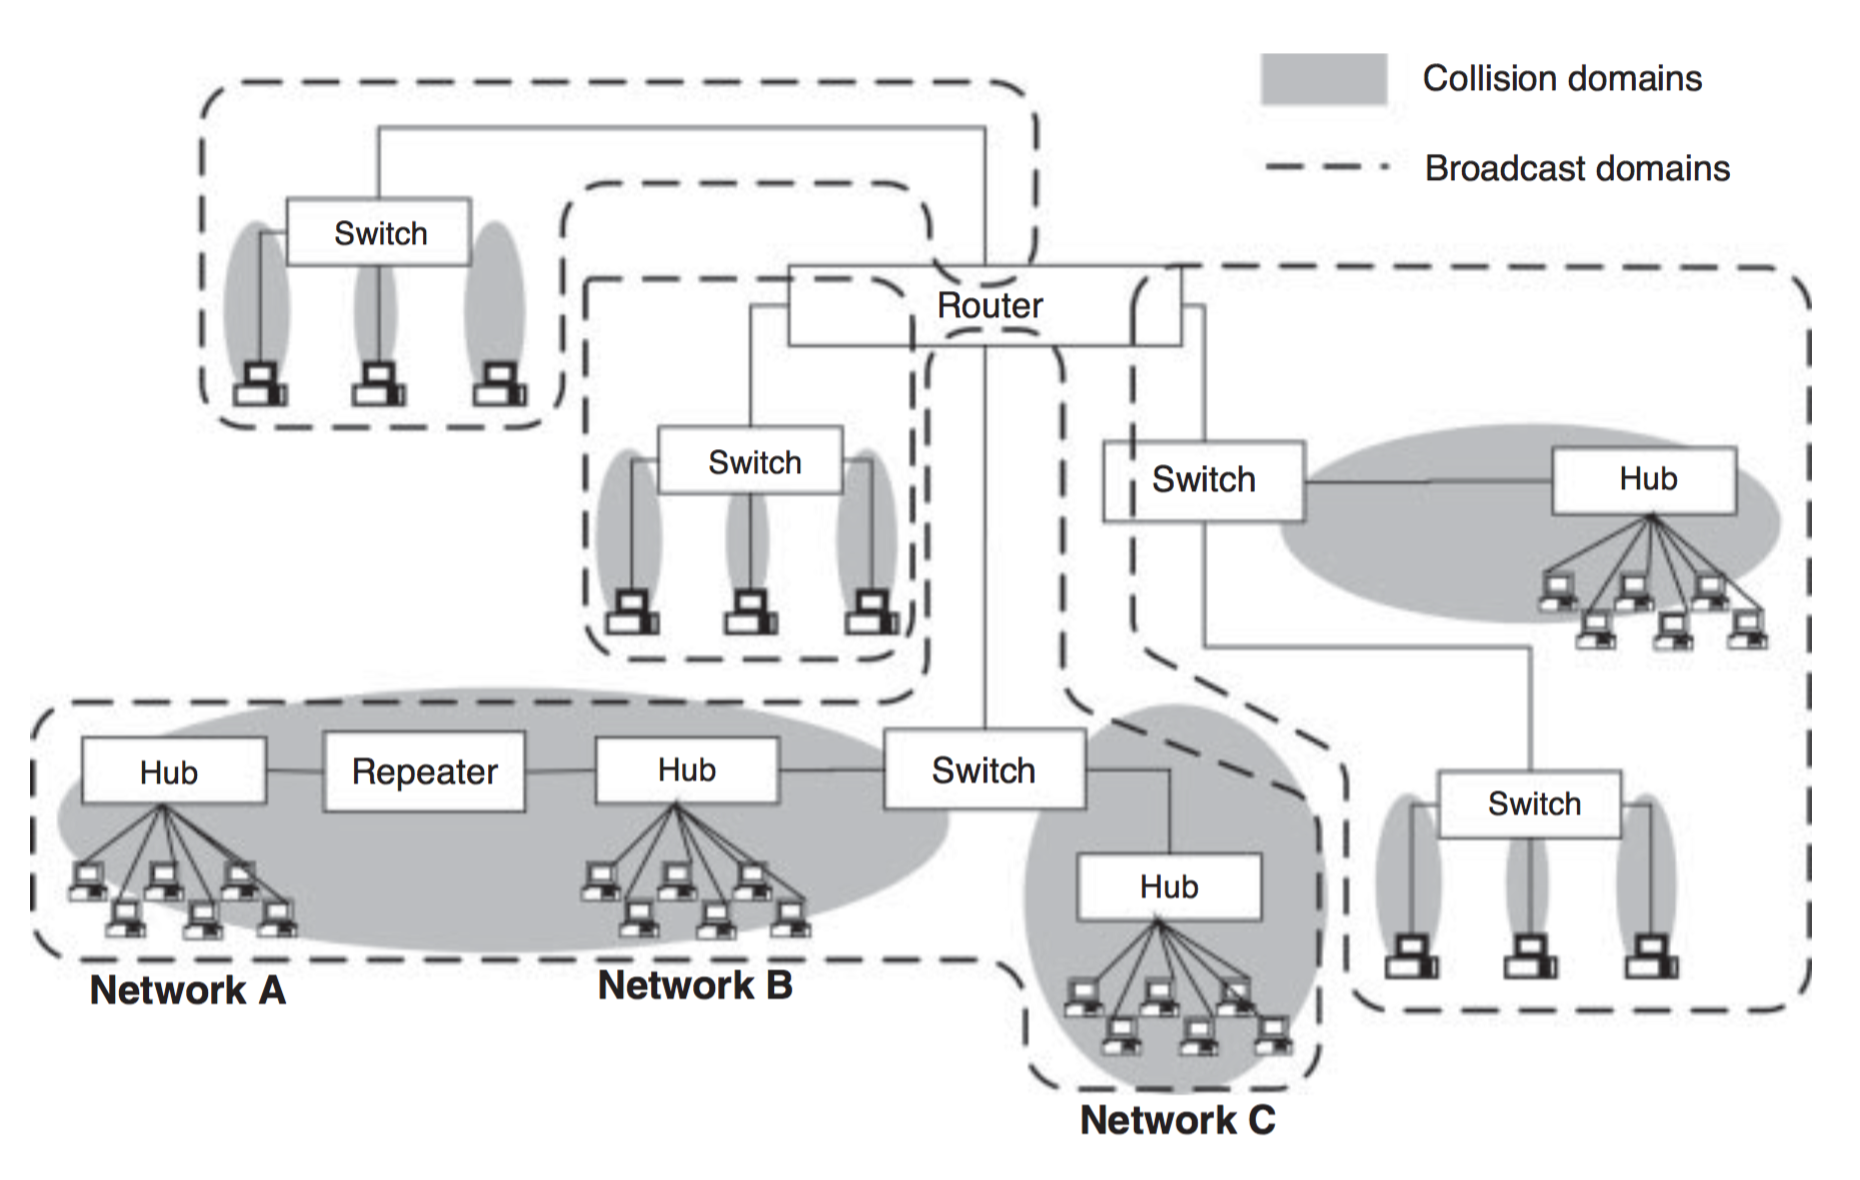
\includegraphics[scale=0.15,cfbox=blue_slides 1pt 0pt]{imgs/lan.png}
	\end{figure}
\end{frame}


\begin{frame}{IEEE 802[.11]}
	\textbf{Wireless}
	\begin{block}{}
	Vic Hayes è stato coinvolto nella progettazione degli standard 802.11a e 802.11b  all'interno di IEEE nel settembre del 1999
	\end{block}
	\pause
	\begin{itemize}[<+- | alert@+>]
		\item Definisce un insieme di standard per le Wireless LAN
		\item Utilizza un mezzo condiviso (collisioni gestite da \textit{CSMA/CA})
		\item Componenti:
			\begin{itemize}
				\item Station
				%Qualsiasi dispositivo che comunica tramite una rete WLAN, ad esempio, un computer portatile, o cellulari che supportano WiFi
				\item Access Point (\textbf{BSS}) 
				%Consente ad una stazione di comunicare con un altra facendo da tramite
				%Gli AP rendono il sistema scalabile e consentono la connessione cablata con altre reti
				%In presenza di AP l’insieme delle station è chiamato Infrastructure BSS
				\item Distribution System (\textbf{ESS})
				%Interconnette Infrastructure BSS attraverso gli AP
				%Facilita la comunicazione tra gli AP, l’inoltro del traffico da un BSS ad un altro ed il movimento di mobile station tra BSS
				%Un insieme di Infrastructure BSS è chiamato Extended Service Set (ESS)
			\end{itemize}
	\end{itemize}
\end{frame}
\begin{frame}{IEEE 802[.11]}
	\textbf{Wireless}
	\newline
	Basic Service Set (BSS)
		\begin{figure}[h] 
			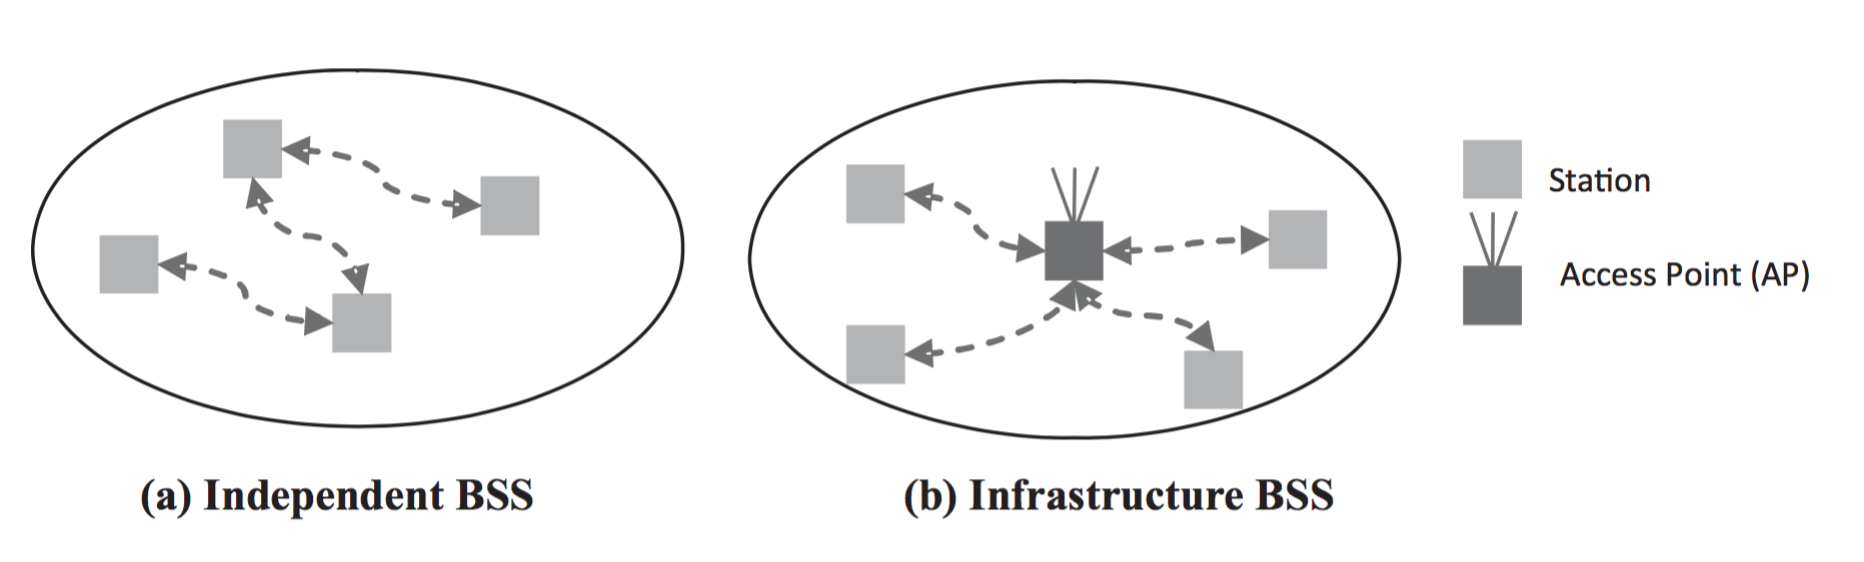
\includegraphics[scale=0.3,cfbox=blue_slides 1pt 0pt]{imgs/bss.png}
			%\caption{Architettura BSS}
		\end{figure}
	\end{frame}
	\begin{frame}{IEEE 802[.11]}
	\textbf{Wireless}
	\newline
	Distribution System
		\begin{figure}[h] 
			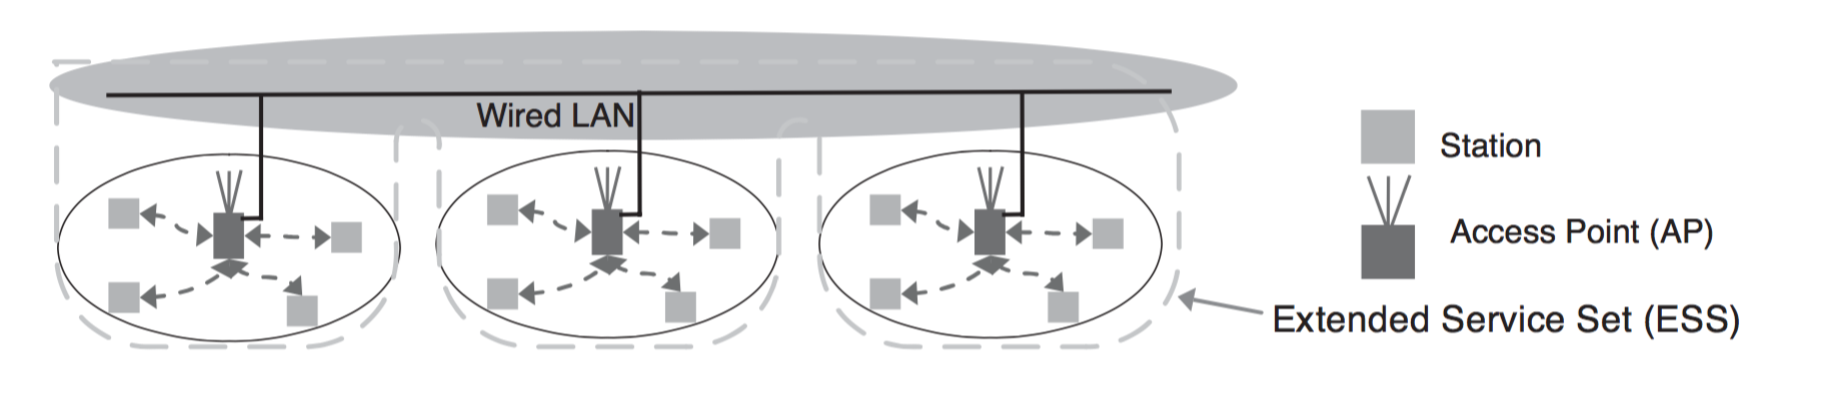
\includegraphics[scale=0.3,cfbox=blue_slides 1pt 0pt]{imgs/ds.png} %border color
		\end{figure}
\end{frame}
	
\begin{frame}{IEEE 802[.15.1]}
	\textbf{Bluetooth}
	\begin{block}{}
		Inventato da Ericsson nel 1994, originariamente concepito come un' alternativa senza fili ai cavi RS-232
	\end{block}
	\pause
	\begin{itemize}[<+- | alert@+>]
		\item Tecnologia wireless progettata per collegare dispositivi mobili o fissi
			\begin{itemize}[<+- | alert@+>]
				\item Bassi consumi
				\item Corto raggio d'azione
				\item Basso costo di produzione per dispositivi compatibili
			\end{itemize}
			\item Presenta due architetture di Rete
			\begin{itemize}[<+- | alert@+>]
				\item Piconet
				\begin{itemize}
					\item Un dispositivo \textit{Master}
					\item Fino a sette dispositivi \textit{Slave}
		%Altri dispositivi possono sincronizzarsi col Master ma non possono partecipare alla comunicazione, tali dispositivi sono in un parked state
		%Un device in parked state può passare in active state se il numero di Slave della Piconet è inferiore a sette
				\end{itemize}
				\item Scatternet
				\begin{itemize}[<+- | alert@+>]
					\item Un insieme di \textbf{Piconet}
				\end{itemize}
			\end{itemize}
	\end{itemize}		
\end{frame}

%	Un dispositivo si può trovare in due stati:
%Connessione: Active mode, Hold mode, Sniff mode, Park mode
%Standby: Ascolta il canale ogni 1,28 secondi per eventuali messaggi dal Master

\begin{frame}{IEEE 802[.15.1]}
\textbf{Bluetooth}
	\begin{figure}[h] 
		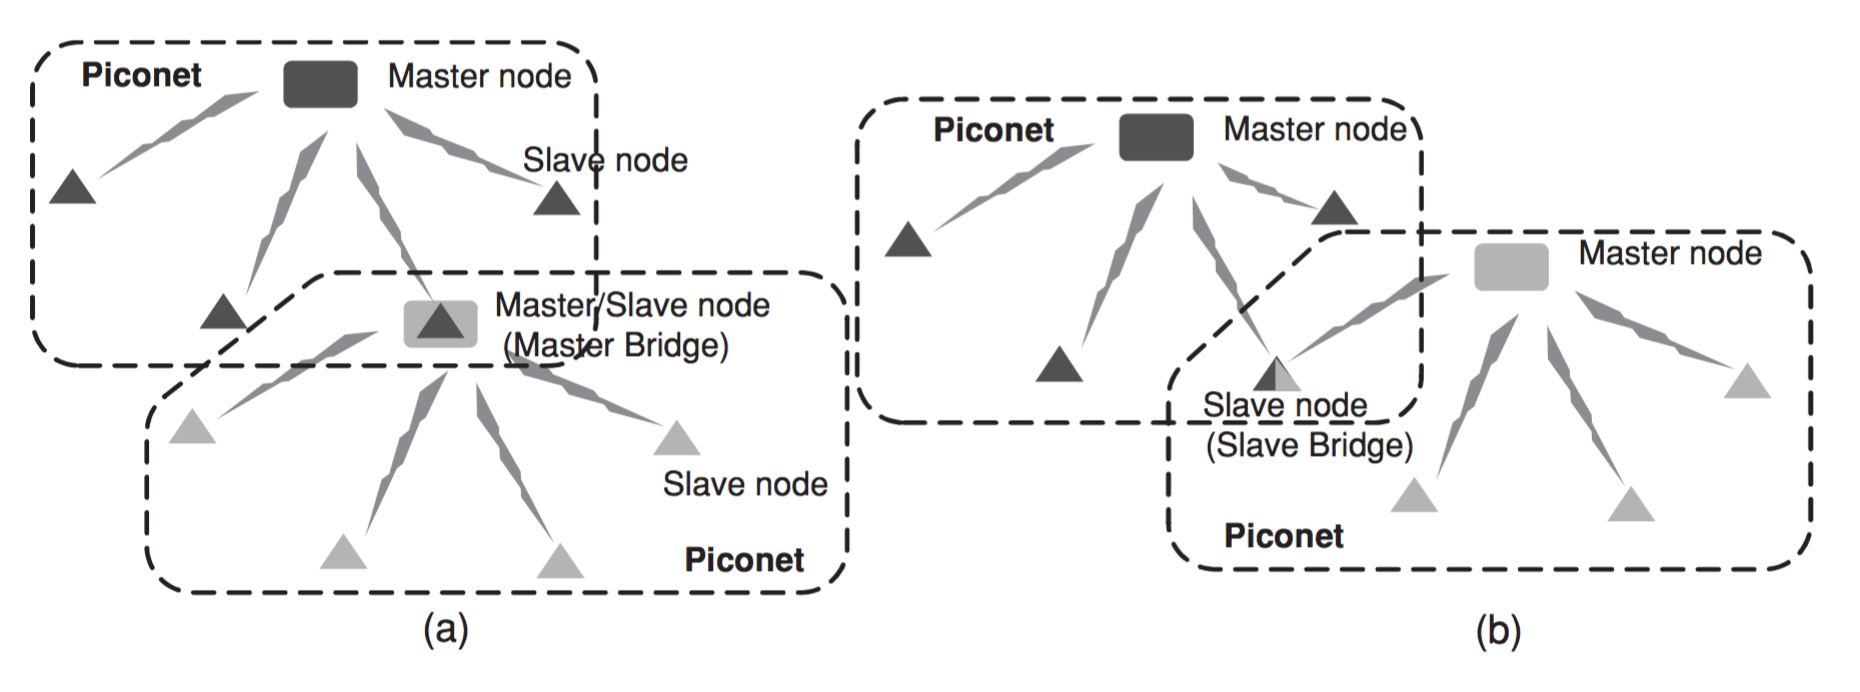
\includegraphics[scale=0.3,cfbox=blue_slides 1pt 0pt]{imgs/bt.png}
		%Le Piconet possono essere interconnesse attraverso un Bridge che può essere Slave per una Piconet e Master per un’altra oppure Slave per due Piconet
	\end{figure}
\end{frame}

\begin{frame}{IEEE 802[.15.4]}
\textbf{ZigBee \& 6LoWPAN}
	\newline
	Sono due tecnologie per Wireless Private Area Network (WPAN)
	\begin{itemize}[<+- | alert@+>]
		\item Basso consumo
		\item Alta flessibilità
		\item Bassi costi
	\end{itemize}
\end{frame}

\begin{frame}{IEEE 802[.15.4]}
\textbf{ZigBee}
\begin{block}{}
La prima specifica fu ratificata il 14 dicembre 2004. La ZigBee Alliance annuncia la disponibilità della specifica 1.0 il 13 giugno 2005%alla quale successivamente vennero rilasciate due versioni nel 2007.
\end{block}
%Considerata come una buona opzione per il metering e per la gestione dell’energia ideale in implementazioni Smart Grid data la semplicità, mobilità, robustezza e i bassi costi di sviluppo.
%Problematiche: basse capacità elaborative, piccola dimensione della memoria e interferenze.
\begin{itemize}
	\item \textit{Application Support} e \textit{Network Layer} sono definiti dalla ZigBee Alliance
	\item Un device può essere di due tipi
	\begin{itemize}
		\item Full Function Device (FFD)
			\begin{itemize}
				\item Coordinatore, Router, Device
				\item Può interagire sia con un FFD che con un RFD
			\end{itemize}
		\item Reduced Function Device (RFD)
			\begin{itemize}
				\item Device
				\item Può interagire solo con un FFD
			\end{itemize}
	\end{itemize}
\end{itemize}
	\begin{figure}[h] 
		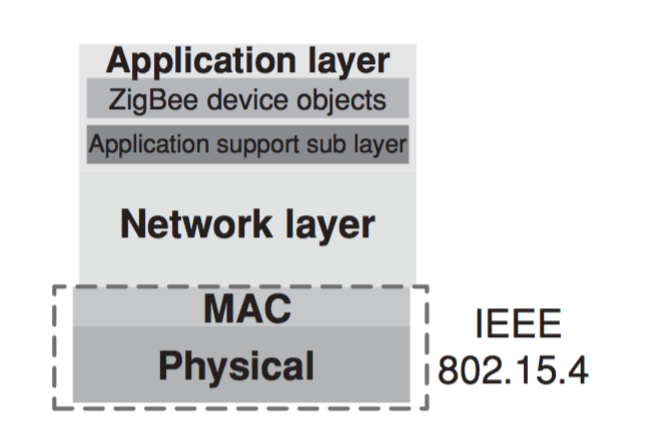
\includegraphics[scale=0.2,cfbox=blue_slides 1pt 0pt]{imgs/zbprot.png}
		%\caption{Architettura protocollare di ZigBee}
	\end{figure}
\end{frame}


%RFD vuole inviare un pacchetto al di fuori del dominio 6LoWPAN.
%RFD -> FFD(router) nella stessa WPAN -> gateway 6LoWPAN che inoltrerà al dispositivo destinatario tramite IP
\begin{frame}{IEEE 802[.15.4]}
	\textbf{6LoWPAN}
	\begin{block}{}
		Il gruppo di lavoro IETF 6LoWPAN è stato approvato nel marzo del 2005. Nel 2009 la ZigBee Alliance ha annunciato l'integrazione di ZigBee con 6LoWPAN
	\end{block}
	\begin{itemize}
		\item Consente l'invio e la ricezione di pacchetti \textit{IPv6}
		\item E' stato inserito un Adaptation Layer per il collegamento tra lo strato \textit{MAC} e il \textit{Network Layer IPv6}
	\end{itemize}
	\begin{figure}[h]
		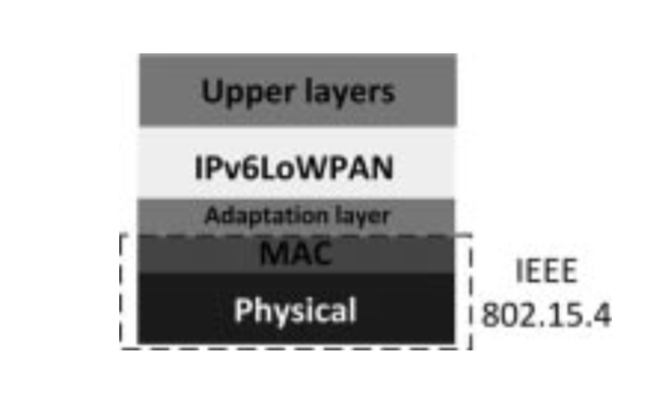
\includegraphics[scale=0.3,cfbox=blue_slides 1pt 0pt]{imgs/6pan.png}
	\end{figure}
\end{frame}

\begin{frame}{IEEE 802[.16]}
	\textbf{WiMAX}
	\begin{block}{}
		Prima pubblicazione effettuata dal WiMAX Forum l'8 aprile del 2002 con lo standard IEEE 802.16-2001
	\end{block}
	\pause
	\begin{itemize}[<+- | alert@+>]
		\item Tecnologia wireless adatta a trasmissione sia di tipo urbano che rurale
		\item Implementa diverse tecniche di crittografia, sicurezza ed autenticazione
		\item Tecnica di Orthogonal Frequency Division Multiple Access (OFDMA)
		\item Soddisfa varie specifiche imposte da una tipica Smart Grid
		%Tra cui massima accessibilità ed interoperabilità, tempi di latenza inferiori ai 50 ms e larghezza di banda di 5 MHz.
		%La copertura si estende fino ai 50 km
		%Supporta i dispositivi mobili
	\end{itemize}
\end{frame}

\begin{frame}{IEEE 802[.16]}
	\textbf{WiMAX}
	\begin{figure}[h]
		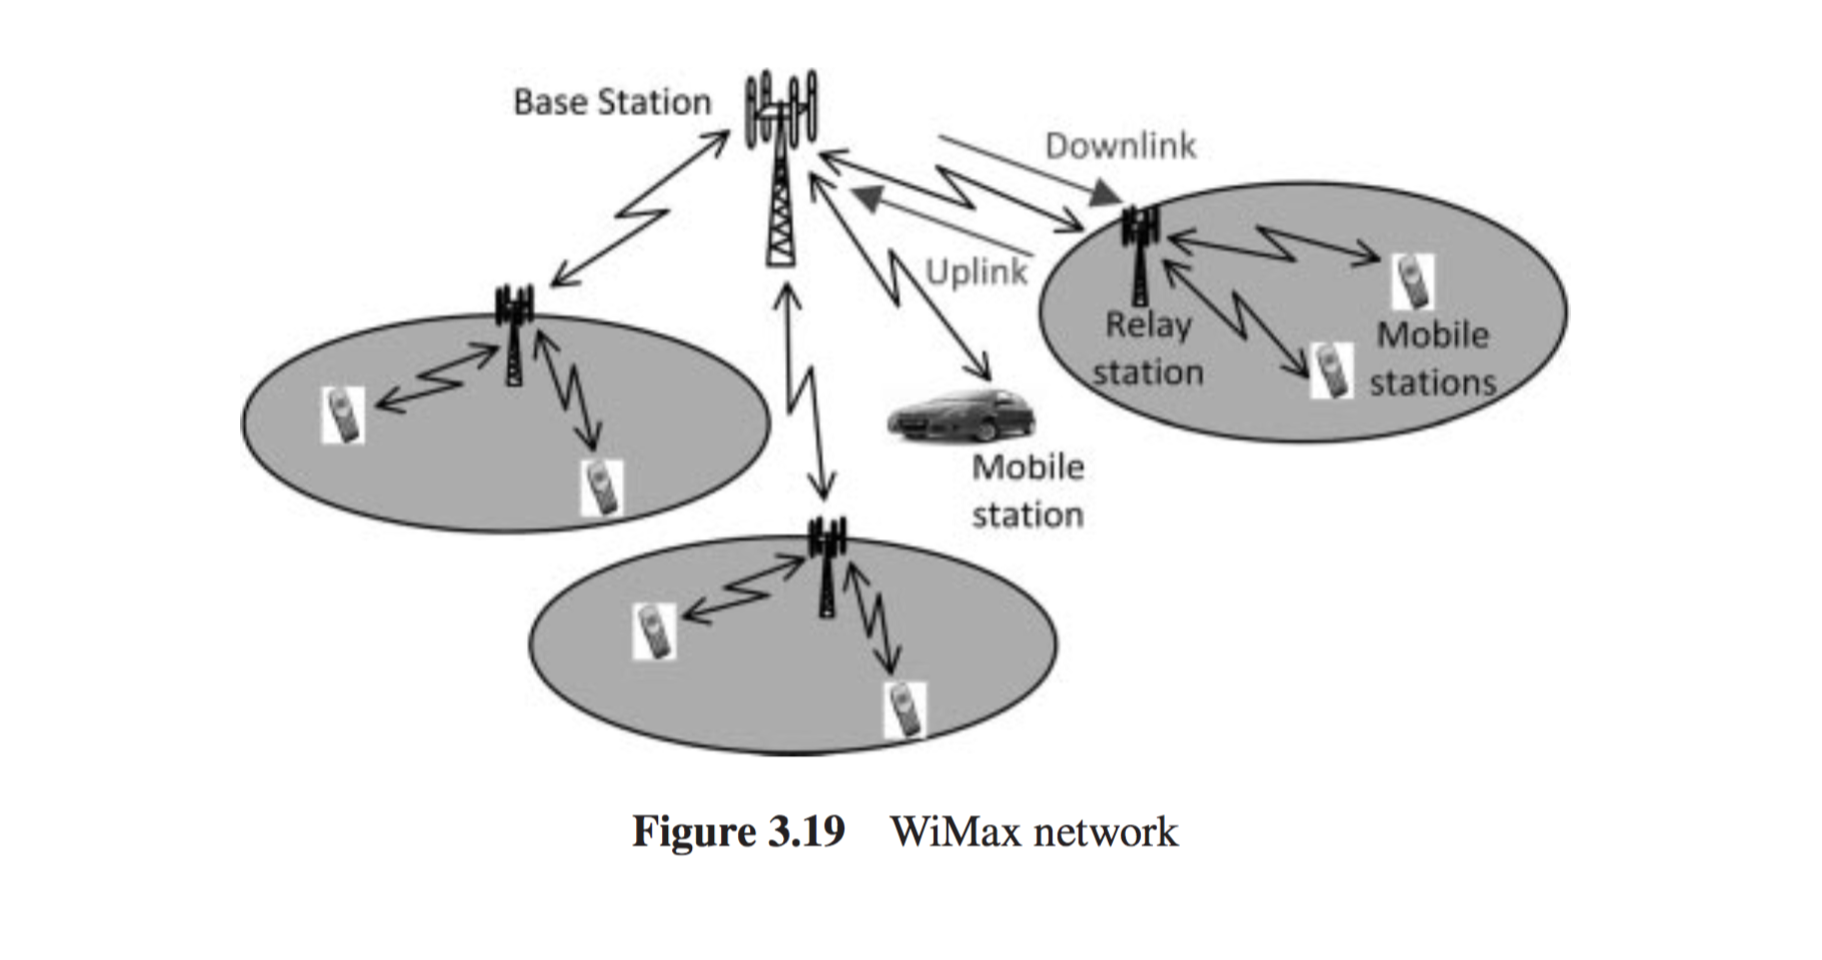
\includegraphics[scale=0.3,cfbox=blue_slides 1pt 0pt]{imgs/wim.png}
	\end{figure}
\end{frame}

%IEEE P1901 e HomePlug
%L’ENEL, nota azienda multinazionale produttrice e distributrice di energia elettrica, ha scelto la tecnologia PLC per trasferire i dati degli smart meter al data concentrator più vicino e la tecnologia GSM per inviare i dati al data center.
%Sono utilizzate tre tecnologie di comunicazione che prendono il nome di narrowband transmission, spread-spectrum transmission e DSP-processed narrowband transmission
\begin{frame}{Power line}
	\textbf{Power Line Communication}
	\begin{block}{}
	I primi standard sono stati progettati nel 2001 dalla Homeplug Powerline Alliance
	%l'Homeplug 1.0 e l'HomePlug 1.0 Turbo, per trasferire dati a una velocità teorica rispettivamente di 15 e 85 Mbit/secondo
	%Dopo alcuni anni di competizione serrata sugli standard, i due standard al di sopra i 200 Mbs sono confluiti in un unico standard internazionale IEEE P1901 Powerline AV, cui rispondono ormai tutti i prodotti in commercio come HPAV Powerline HomePlug AV
	\end{block}
	\pause
	\begin{itemize}[<+- | alert@+>]
		\item Tecnologia di rete proposta per la trasmissione in ambiente Smart Grid
		\item Trasporto informazioni su conduttori e linee elettriche %risparmio dal punto di vista di creazione dell'infrastruttura
		\item Servizi di comunicazione per AMI e HAN
	\end{itemize}
	\pause
	\begin{block}{}
		\textit{In una tipica rete \textbf{\color{blue_slides}PLC}, gli smart meter sono collegati al data concentrator attraverso power line e i dati vengono trasferiti al data center tramite tecnologie di rete cellulare}
	\end{block}
	\pause
	\begin{block}{Problema}
		Presenza di disturbi che possono corrompere le informazioni, non garantendo più la continuità del servizio
	\end{block}
\end{frame}

\plain{Standard per lo scambio di informazioni}

%DNP3
%Insieme di protocolli di comunicazione utilizzato tra i componenti nei sistemi di automazione
%Fondamentale nei sistemi SCADA, utilizzato dalle Master Station per comunicare con le RTU e gli IED
%	Lo User Layer DNP prende input analogici/binari e da in output segnali analogici e binari.
%Un master dnp3 invia richieste e le stazioni Slave rispondono, ma uno Slave può anche trasmettere messaggi senza aver ricevuto richiesta.
%Il Physical Layer utilizza noti protocolli di comunicazione seriali come EIA 232 o EIA 485.

\begin{frame}{Standard per lo scambio di informazioni}
	\textbf{Modbus}
	\begin{block}{}
	Protocollo creato nel 1979 da Modicon (azienda ora parte del gruppo \textbf{\color{blue_slides}Schneider Electric})
	\end{block}
	\pause
	\begin{itemize}[<+- | alert@+>]
		\item Protocollo di messaggistica (\textit{Application Layer})%risiede nell’Application Layer e consente la comunicazione tra i dispositivi collegati su diversi bus e reti
		\item Dispositivi collegati su diversi bus e reti%protocollo utilizzato per mettere in comunicazione i controllori logici programmabili
		\item Ethernet su fibra ottica con trasmissione seriale asincrona%EIA 232, EIA 422, EIA 485
		\item Automazione delle substation%Modbus su EIA 485
		\item Comunicazione
			\begin{itemize}[<+- | alert@+>]
			\item Master $\xrightarrow{query}$ Slave/broadcast
			\item Slave (monitoring delle \textit{query})
			\item Slave $\xrightarrow{trigger}$ azione
			\end{itemize}
	\end{itemize}
\end{frame}


%Generalmente, questi protocolli girano su reti TCP/IP o LAN con switch Ethernet molto performanti per rispondere ai requisiti stringenti dei dispositivi, che necessitano di tempi di risposta inferiori a 4-5 millisecondi.
\begin{frame}{Standard per lo scambio di informazioni}
	\textbf{ISO/IEC 61850}
	\begin{block}{}
		Un gruppo IEC di 60 membri si è diviso in 3 gruppi di lavoro per la creazione di ISO/IEC 61850 nell'1995
	\end{block}
	\pause
	\begin{itemize}[<+- | alert@+>]
		\item Progettazione dei sistemi di automazione per le substation
		\item Sovrastruttura che coordina e gestisce protocolli e tecnologie esistenti
		\item Garantisce interoperabilità
	\end{itemize}
\end{frame}

\begin{frame}{Standard per lo scambio di informazioni}
	\textbf{ISO/IEC 61850}
	\begin{block}{Vantaggi}
	\begin{itemize}[<+- | alert@+>]
		\item Coordina la complessità di unità indipendenti
		\item Si integra con sistemi preinstallati in rete
		\item Scalabile e facilita integrazione
		\item Si basa su standard esistenti
		\item Supporta i \textit{self descriptive device}%eliminando problemi di configurazione manuale
		\item Si basa su \textit{data object}%e standardizzazione degli elementi tipici di una rete elettrica
		\item Estensibile e flessibile
		\item Si adatta rapidamente alla configurazione del sistema
	\end{itemize}
	\end{block}
\end{frame}

%ISO/IEC 61850 suddivide ogni sottostazione in tre livelli[25] chiamati Station Level, Bay Level e Process Level

%Un device model considera inizialmente un physical device. Tale modello consente ad un singolo dispositivo fisico di agire da gateway di informazioni per più dispositivi. Successivamente vengono specificati i logical device all’interno di tale dispositivo. Ogni logical device contiene uno o più logical node, logicamente correlati ad una funzione della stazione. I logical node sono definiti da gruppi di data object e relativi servizi, ognuno modellato secondo gli schemi definiti dalle Common Data Classes (CDC).

%I logical node sono identificati con nomi definiti dallo standard in cui la prima lettera indica l’attinenza (e.g. A controllo automatico, M misura, X switchgear, etc)

%Utilizzando tale formato si è in grado di indicare le informazioni relative allo status o alla posizione di un dispositivo
\begin{frame}{Standard per lo scambio di informazioni}
\textbf{ISO/IEC 61850}
	\newline\textbf{Device Model}
	\begin{figure}[h] 
		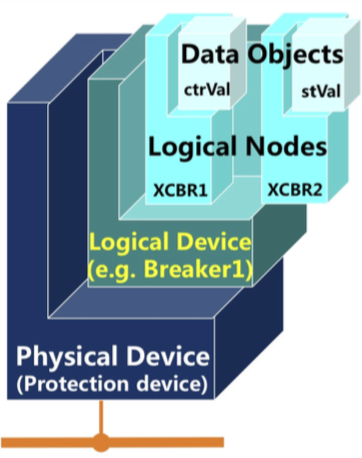
\includegraphics[scale=0.35,cfbox=blue_slides 1pt 0pt]{imgs/iec61850ln.png}
	\end{figure}
\end{frame}

\begin{frame}{Standard per lo scambio di informazioni}
\textbf{ISO/IEC 61850}
	\begin{itemize}[<+- | alert@+>]
		\item Oggetti e servizi astratti di comunicazione %permettono di scrivere un'applicazione indipendentemente dai protocolli tradizionali.
		\item Abstract Communication Service Interface (ACSI)
			\begin{itemize}[<+- | alert@+>]
				\item Oggetti e servizi implementati attraverso il protocollo Manufacturing Message Specification (MMS) 
				%Che definisce i messaggi di comunicazione tra i centri di controllo o tra stazioni e centri
			\end{itemize}
		\item Linguaggio comune di configurazione per astrazione e standardizzazione
		\begin{itemize}[<+- | alert@+>]
			\item Substation Configuration Language (SCL)%basato su XML
			\begin{itemize}[<+- | alert@+>]
			\item[+] Interoperabilità tra IED
			\item[+] Configurazione automatica
			\item[+] Riduzione della presenza di errori
			\end{itemize}
			\item Ogni IED presenta un file SCL che ne definisce la configurazione
		\end{itemize}
	\end{itemize}		
\end{frame}

\begin{frame}{Standard per lo scambio di informazioni}
\textbf{ISO/IEC 61850}
\newline
Lo standard si serve dei seguenti strumenti per la gestione delle informazioni
\begin{itemize}[<+- | alert@+>]
	\item Generic Substation Event (GSE)
	%Protocollo che fornisce uno strumento veloce ed affidabile per la segnalazione di eventi all’interno della sottostazione. Le caratteristiche principali sono il servizio multicast/broadcast con modello di comunicazione publish/subscribe. I messaggi sono trasmessi in formato binario. GSE prevede due modelli di servizio che prendono il nome di GOOSE e GSSE
	\begin{itemize}[<+- | alert@+>]
		\item Generic Object Oriented Substation Event (GOOSE)
		%Utilizza Virtual LAN, stabilendo più network virtuali sulla stessa rete fisica e determinando livelli di priorità per i messaggi, consentendone anche la ritrasmissione
		\item Generic Substation State Event (GSSE)
		%Utilizzato per lo scambio di informazioni sui soli cambiamenti di stato. In questo caso i messaggi sono costituiti da una serie di bit che rap- presentano liste di stati. GSSE necessita un tempo di trasmissione maggiore se confrontato con GOOSE
	\end{itemize}
	\item Sampled Measured Values (SMV)
	%Protocollo per lo scambio di dati e la trasmissione di misure prodotte dai trasduttori delle sottostazioni: permette lo scambio di segnali tra gli IED
	\item Time Synchronization
	%Servizio di sincronizzazione dei clock fondamentale per applicazioni real-time. Utilizza un subset di Network Time Protocol (NTP) con riferimento allo Universal Coordinated Time (UTC). NTP è il protocollo tipicamente utilizzato per sincronizzare i clock di computer collegati ad Internet e in LAN.
	\item Report e Logging
	%REPORT: Strumento che permette di memorizzare i cambiamenti dei dati e degli attributi relativi ai nodi logici. Genera dataset contenenti attributi di interesse e richiede ai nodi logici l’invio delle informazioni riguardanti le variazioni nel sistema
	%LOG: Registrazione degli eventi relativi ad un dispositivo. I log sono registrati in un server e, a differenza dei Report, i dispositivi logici creano al loro interno un database di eventi senza inviarne notifica
\end{itemize}
\end{frame}

\plain{Standard per la sicurezza}

%Di recente invenzione e fondamentali data la grande mole di informazioni sensibili memorizzate sui computer collegati in rete
%Molte attività si sono automatizzate introducendo maggiore bisogno di affidabilità e sicurezza

%Limiti di ISO/IEC 61850: costi elevati per l’installazione dei server e dei dispositivi atti alla gestione dei dati ma anche complessità dal punto di vista dell’architettura
%ISO/IEC 61850 è affiancato da ISO/IEC 62351 che garantisce la sicurezza e specifica i requisiti tecnici che devono essere rispettati dai fornitori

\begin{frame}{Standard per la sicurezza}
	\begin{block}{I problemi relativi alla sicurezza}
	\begin{itemize}
		\item[-] Accessi non autorizzati a informazioni recuperate dagli smart meter
		\item[-] Spegnimento di dispositivi
		\item[-] Attacco alla Smart Grid per causare un'interruzione al regolare passaggio di corrente
	\end{itemize}
	\end{block}		
	\pause
	\begin{block}{I problemi relativi alla privacy}
	\begin{itemize}
		\item[-] Alta frequenza di letture per misurare il consumo energetico
		\item[+] Si cerca di aggregare le informazioni per mascherare i singoli consumi dei meter
	\end{itemize}
	\end{block}		
\end{frame}

\begin{frame}{Standard per la sicurezza}
\textbf{ISO/IEC 62351}
\begin{block}{}
Standard sviluppato nel 1999 dal WG15 facente parte della TC57 dell'organo internazionale IEC
\end{block}
\pause
\begin{block}{Obiettivi di sicurezza}
\begin{itemize}
	\item Autenticazione nel processo di trasferimento di dati tramite firma digitale
	\item Garanzia di accessi esclusivamente dopo autenticazione
	\item Prevenzione dell'\textbf{\color{blue_slides}eavesdropping}%ossia intercettazioni della comunicazione non autorizzate
	\item Prevenzione da attacchi di \textbf{\color{blue_slides}playback} e attacchi di \textbf{\color{blue_slides}spoofing}
	%PLAYBACK (REPLAY ATTACK): Impossessarsi di una credenziale di autenticazione comunicata da un host ad un altro, e riproporla successivamente simulando l'identità dell'emittente	
	%SPOOFING: ovvero sostituirsi ad una controparte della comunicazione
	\item Rilevamento delle intrusioni
\end{itemize}
\end{block}
\end{frame}

\begin{frame}{Standard per la sicurezza}
	\textbf{ISO/IEC 62351}
	\newline
	E'suddiviso in 8 parti:
	\begin{enumerate}[<+- | alert@+>]
		\item Spiegazioni di alcuni scenari
		\item Definizioni di termini
		\item Definizioni di servizi di sicurezza in comunicazione TCP/IP based
		%Definisce come possono essere forniti servizi di sicurezza in una comunicazione TCP/IP based e specifica suite di cifratura
		\item Aumento dei messaggi di sicurezza trasmessi su MMS
		%Definisce procedure, i miglioramenti del protocollo, e gli algoritmi atti a promuovere l’aumento dei messaggi di sicurezza trasmessi su MMS
		%Tali procedure sono relative a Transport e Application Layer, basate su TLS, usate in modo da proteggere le informazioni trasmesse
		\item Comunicazione seriale
		%in cui si vanno a definire ulteriori misure di sicurezza per proteggere l’integrità delle connessioni seriali applicando chiavi hash
		\item ISO/IEC 61850 %profili iso/iec 61850 per la comunicazione non basati su TCP/IP
		\item Network Management%implementa o estende sistemi di intrusion detection
		\item Role-Based access control
		%Approccio a sistemi ad accesso ristretto per utenti autorizzati.
		%Tre regole fondamentali sono definite per il modello RBAC: Assegnazione dei ruoli, Autorizzazione dei ruoli, Autorizzazione alla transazione
	\end{enumerate}
\end{frame}